\documentclass[thesis.tex]{subfiles}

\begin{document}

\chapter{Background}

 Every now and then I get the question ``what is it you do, anyway?'' Often enough the question is posed out of sheer politeness, and I can simply say ``Physics! Tiny particles, like plankton, they tumble in the oceans, and stuff.'' But sometimes the question is sincere, and I find that it is quite a challenge to explain to a non-expert. I may say that we calculate how non-spherical particles rotate in flows. But that is comparable to if I was designing a gearbox, and said that I work with cars. It is true, but not very helpful. The following is an attempt at a description which is readable and not too complicated, but still complicated enough to get a glimpse of the physics.


\section{Our field of study: particles in flows}\label{sec:context}

Where do particles go when I put them into a flow? Which way do they face, how fast do they spin? These are all valid questions, but they are unspecific. Of course the answers depend on if the particle is an aircraft or a grain of particulate carbon soot, and if the liquid is air or water. 

In the following pages, I will try to tell a story, with the intention that you form an image of the physics we study. I will start with an elaboration on fluid physics, move through why we consider rigid particles specifically, then say something about the forces acting on the particles. This will naturally lead us to why we must consider ``small'' particles, which is not obvious from the outset.

\subsection*{Fluids}

Many physical systems around us are fluids. The air we breathe, the water we drink, the blood in our veins are all fluids. As a working definition we can think of a fluid as a system where the constituent molecules move around more or less freely. Sometimes they interact with each other and exchange some energy. The collisions give rise to what you perceive as friction. You know that syrup has more friction than water: if you pull a spoon through syrup, more of your energy is expended colliding molecules than if you were to pull the spoon through water. A measure of how often and how violently the molecules collide is the \emph{viscosity} of a fluid, and we say that syrup has higher viscosity than water. Now, it gets interesting when something else, for example a drop of oil or a particle, is added to the fluid. Consider dripping a drop of oil into water. Then what happens depends on how the water molecules interact with the oil molecules. As you probably have experienced, the oil molecules prefer to stick together. Therefore the oil concentrates into a drop where as many oil molecules as possible may be neighbours with other oil molecules.

But so far, the above is a very qualitative, and you may rightly say naive, description of what happens. One could say that a fundamental problem of fluid physics is to figure out where all the different molecules go. From the detailed knowledge of every molecule we may proceed to deduce where the oil drop goes, and how fast, or if it perhaps breaks up, or maybe merges with another drop. However, making something useful out of this molecular picture is very difficult\footnote{
%\begin{minipage}[l]{\textwidth}
However, modern computers now allow simulation of surprisingly large numbers of molecules. Here is a video showing the interface between two molten metals using exactly this approach. \url{http://www.youtube.com/watch?v=Wr7WbKODM2Q}
 %\end{minipage}
% \begin{minipage}[l]{1.5cm}
% 
\includegraphics[width=1.5cm]{figs/ninebillion_qr.png}
% \end{minipage}
}.
Just consider that in one litre of water there are about $10^{25}$ molecules (that is a very large number; about the weight of the Earth in kg). In fact, we are not even particularly interested in the specific details of every molecule - we are interested in the macroscopic, observable world that is built up from all these molecules. Now, this thesis is not at all concerned with the detailed motion of molecules, but I still wanted to start with this picture because sometimes it becomes important to remember the origin of the macroscopic motion.

%\todo{connect forward to chap's about noise, fokker-planckery}.

\subsection*{Fluid dynamics}

The discipline studying the macroscopic properties and motion of fluids is called fluid dynamics. Some typical quantities studied there are the fluid velocity and pressure. We can think of the velocity at a certain position in the fluid as the average velocity of all the molecules at that point. The pressure is the force per area an object in contact with the fluid experiences, due to the constant bombardment of molecules. Think for example of the forces in a bottle of soda. There are well-known equations called the Navier-Stokes equations (you can see them in \Eqnref{navierstokes} on p.~\pageref{eqn:navierstokes}) which describe the velocity and pressure, if we can solve them. We will soon return to how this helps us, but first we must restrict ourselves to avoid a difficult hurdle.

Recall our example of a drop of oil in water. The switch from a molecular view to a fluid dynamical view opens a new problem: if we do not keep track of every molecule, we instead have to keep track of which points in space contain oil and which contain water. Separating the two materials, there is a boundary surface which can deform over time as the oil drop changes shape. This sounds very complicated. Indeed, drop dynamics is a topic of its own, which this thesis does not intend to cover. Instead, this thesis concerns \emph{rigid particles}.

\subsection*{Rigid bodies}

A rigid body in physics is an object whose configuration can be described by the position of one point (usually the center-of-mass) and the rotation of the body around that point. Simply put: it cannot deform. The dynamics of a rigid body is described by Newton's laws. In particular, the center-of-mass motion is described by the famous relation that the force $\ve F$ on a body equals its mass $m$ times its acceleration $\ve a$,
\begin{align*}
	\ve F = m\ve a.
\end{align*}
While the above equation describes the movement of the position, there is a corresponding law for the rotation. Since this thesis concerns \emph{orientational dynamics} of particles, we need equations also for the rotation of a rigid body. Newton's law governing rotations says that the torque $\ve T$ on a rigid body equals its moment of inertia $\ma I$ times its angular acceleration $\ve \alpha$,
\begin{align*}
	\ve T = \ma I \ve \alpha.
\end{align*}
The two equations above are deceivingly simple-looking, but their solutions contain full knowledge of the motion of a rigid body. I state the equations here only to draw a conclusion: in order to extract all the information about the motion of a particle, we need to know both the force and the torque acting on the particle at all times.

There are many kinds of forces which can potentially act on a particle. For example there is gravity if the particle is heavy, or magnetic forces if the particle is magnetic. But for now we consider the forces on a particle due to the surrounding fluid, so called hydrodynamic forces. In everyday terms the hydrodynamic force is the drag, as experienced by a car for example. Uneven drag over a body may also result in a hydrodynamic torque. For instance, turbulent air striking the wings of an aircraft will induce a torque which you feel as a rotational acceleration while the pilot compensates.

\subsection*{Hydrodynamic forces}

In order to find out what the force on a particle is, we need to know how the fluid around the particle behaves. And for that, we need to solve the Navier-Stokes equations of fluid dynamics around the particle. What does it mean to ``solve'' the equations? We imagine the fluid in some environment (we call this ``boundary conditions''), for example the air in a cloud. A solution of the equations tells us for example the velocity of the fluid at any given point at any given instant. If we have a solution, we know how to extract the resulting forces and torques on a particle in the fluid.

The problem is that we cannot solve the equations. Not only can we not find solutions as mathematical formulas - in many cases we can not even find numerical solutions using a supercomputer.For example, computing the motion of the air in a cloud is utterly out of reach with the computer resources of today. 
I think it is worthwhile to emphasise that some problems are inherently very hard, and cannot be solved by brute force. From time to time I get the question why we struggle with difficult mathematical work, why not just ``run it through the computer?'' A numerical computer solution is like an experiment: it will give you the numbers for a particular case, but not necessarily any understanding of why. We aim to extract all possible physical understanding available from the equations, even if it not possible to solve them in general. It is the understanding of the underlying physics that enables us to simplify the equations until it is practical to solve them. This requires knowledge of which particular details may be neglected, and which details are crucial to keep track of. 

And indeed, the meteorologists now have methods of simulating the flows of air in the atmosphere. The trick is to ignore parts of the equation dealing with very small motions, and spend the resources on describing the large eddies of the flow, it is called ``Large Eddy Simulations''. The game of simplifying without over-simplifying is at the heart of fundamental research.

At any rate, we wish to figure out what the forces on a rigid body in a fluid flow are. By now it is clear that some type of simplification has to be made. The great simplification is embodied in the word \emph{small} in the title of this thesis. The particles we consider are small. But how small is a small particle? The answer I have to give right away is a rather unsatisfactory ``it depends''. The smallness of the particle has to be relative to something else. This simple principle is formalised by scientists, who discuss smallness in terms of \emph{dimensionless numbers}. Because dimensionless numbers are very common in our work I will spend a few paragraphs to explain the basic idea.

\subsection*{Dimensionless numbers}

In principle all physical quantities have some units. For example, the size of a particle has units of ``length'', and the speed of the particle has units of ``length per time'', which we write as \nobreak{length/time}. Whenever we multiply or divide quantities with dimensions, we also multiply or divide their units. For example dividing the length \unit[20]{m} with the time \unit[5]{s} gives the speed \unit[4]{m/s}. Now suppose we divide the speed \unit[4]{m/s} with the speed \unit[2]{m/s}. The result is $2$, without any units - they cancelled in the division. The idea is that in order to determine if a quantity $x_1$ is ``small'' we have to divide it with another quantity $x_2$ of the same units. Then if the resulting dimensionless number is smaller than $1$, we say that $x_1$ is small, and implicitly mean \emph{relative to $x_2$}.  This concept seems simple enough, let's consider a slightly more complicated example.

Imagine a small rubber boat on the sea. There are waves on the sea, rising and falling periodically.  The boat speeds along, also rising and falling as it crosses the waves. Now I propose to find a dimensionless number that tells us if the boat is ``fast''. So it has to be fast relative to something else, and the only thing we know of are the waves. 

There are two distinct mechanisms at play for the rising and falling of the boat. First, if the boat stays in a fixed position the sea will rise and fall beneath it periodically. Call this period time $\tau$. Second, the boat may cross different waves by travelling over them. Let's call the speed of the boat $v$, and the distance between different waves on the sea is a length $\eta$. In the paragraph above we concluded that we have to divide $v$ with another speed, and check if the dimensionless number is smaller or larger than $1$. With the quantities we know of, that is the wave period time $\tau$, the wave distance $\eta$ and the boat velocity $v$, there is only one dimensionless combination. We can divide the speed $v$ with the speed $\eta/\tau$. The ratio is a number which I will call the \emph{Kubo number}, for reasons I will explain shortly. The Kubo number is
\begin{align*}
\ku = v\tau/\eta.
\end{align*}
I will now give a brief interpretation of what it means when $\ku$ is smaller or larger than $1$. If $\ku > 1$, it means that $v\tau > \eta$. The quantity $v\tau$ is a length, more precisely the length that the boat travels during the period time of a wave. Thus, $\ku > 1$ means that the boat travels more than one wave distance during the period time of a single wave. So when the Kubo number is very large, then the boat travels over many different waves before the wave landscape changes. In this case we may rightly say that the boat is \emph{fast}. On the other hand, if $\ku<1$, the boat does not cover the distance between waves in a single wave period time. Before the boat reaches the next wave, the entire wave landscape has changed underneath it.

I made this example of the Kubo number because it is one of the fundamental quantities in Paper~C, which is about rotation rates of particles in turbulence. There a particle plays the role of the boat, and a turbulent flow plays the role of the waves. As I did here, we there describe the limits of very small $\ku$, and very large $\ku$. In a real turbulent flow $\ku$ is around $1$. That is to say neither of the extremes are true, but in the paper we argue that together they bring some insight into the tumbling of the particles. The usage of dimensionless numbers simplifies our work. Instead of considering the effects of all three separate parameters, we can understand the physics by analysing a single dimensionless number.

The dimensionless numbers tell us which physical quantities are important in relation to each other. In the example above, the actual speed of the boat is not important - the speed only matters in relation to the waves. We know that all situations with the same Kubo number are, in some sense, equivalent. This very fact is also what enables engineers to use scale models in wind tunnels. They know that to test a model of a suspension bridge in a wind tunnel, they can not use full-scale wind speeds, but instead a scaled down version of the wind. The dimensionless numbers reveal what scaling is appropriate to match the model bridge to real conditions.

\subsection*{Small particles}

We are now equipped to understand what it means for a particle to be \emph{small} in the context of fluid flows. It turns out, in our setting, that there are two dimensionless numbers that determine whether a particle is small. One has to do with how quickly the particle adjusts to the fluid, the other with how quickly the fluid adjusts to the particle.

The first dimensionless number is the Stokes number, $\st$ for short. We can understand it as a comparison of two different time scales. The first is the time it takes for the particle to stop if thrown in an otherwise still fluid. If you throw a stone in air, it takes quite some time for the drag force to stop the stone. But if you try to throw a piece of paper, the drag force overcomes the inertia almost immediately. On the other hand, if you try to throw the stone under water, the time to stop is shorter than in air. We call this time the relaxation time of the particle in the fluid. The relaxation time of the particle is compared to how quickly the fluid velocity changes. In summary, 
\begin{align*}
 	\st = \frac{\textrm{Particle relaxation time}}{\textrm{Time for fluid velocity change}}.
 \end{align*} 
A small Stokes number means that the particle adjusts to the fluid faster than the fluid changes. Such particles stick closely to the flow velocity. Conversely, a large Stokes number means that the fluid changes before the particle has time to adjust, and the particle is relatively unaffected by the fluid velocity. Thus the first meaning of a \emph{small} particle is in the sense that the Stokes number is small, and the particle relaxes to the surrounding drag forces before they change.

The other dimensionless number measuring particle smallness is the particle Reynolds number. It is a measure of how quickly disturbances in the flow settle down. If you stir with a spoon in your cup of tea there is a wake behind the spoon, perhaps even a vortex is created. When you stop stirring, the tea will splash about for a moment and then settle down. The time it takes for a small vortex to settle down is called the viscous time, because it is related to the viscosity of the fluid. Imagine stirring with a spoon in syrup instead of tea, the wake behind the spoon relaxes more quickly in the viscous fluid. But of course it also matters how vigorously you stir, or equivalently, how fast the fluid moves relative to the spoon. To find the particle Reynolds number we compare the viscous time to how fast the spoon, or particle, moves the distance of one particle length:
\begin{align*}
 	\rep = \frac{\textrm{Viscous time}}{\textrm{Time for fluid to flow one particle length}}.
 \end{align*} 
A small particle Reynolds number implies that the viscous time is short, and the fluid disturbances we create settle down before the fluid has time to move past the particle. A large particle Reynolds number means that the vortices and disturbances produced by the particle are transported away from the particle, like the wake and vortices you observe in your cup of tea. The second meaning of a \emph{small} particle is that the particle Reynolds number is small, so that there is no wake, and no vortices created by the particle. 
Recall the story about the Stokes drag in the very beginning of this thesis. When Stokes in 1851 called a particle ``slowly moving'', he meant exactly the condition that the particle is small, in the sense just described here.

\subsection*{Summary}

Hopefully we have established enough common ground to put the appended research papers in context. The presentation in Part~II may, or may not, be too technical for the casual reader. But even if, I hope I may encourage an ever so brief look.

At the very least, we have a working interpretation of the technical title ``Orientational dynamics of small non-spherical, rigid particles suspended in fluid flows.'' The interpretation is that we aim to understand the rotational motion of a non-spherical rigid body immersed in a fluid bath of molecules. We know the forces and torques driving the rotation through the macroscopic description of fluid dynamics. But in order to have a fair chance at progress, we consider the case of very small particles, as characterised by the Stokes and particle Reynolds dimensionless numbers.


\chapter{Prerequisite concepts}

In this section I will introduce the basic concepts needed to understand the appended research papers. 

\section{Forces on particles in fluids}\label{sec:forces}

We are studying the dynamics of small particles suspended in flows. Specifically, we consider particles small enough to not create disturbances in the fluid flow. In such cases, one can consider the fluid flow as a prescribed input, and calculate the response of the particles. Obviously, the particle will disturb the flow -- in fact, it is the reaction force of this disturbance which acts on the particle.
What I mean is that the particle does not induce long-lived disturbances in the fluid now, which survive to affect the particle at a later time. In order to understand this requirement, and how the particle forces are calculated, we will start at the Navier-Stokes equation.

The governing equation for an incompressible, Newtonian fluid is the Navier-Stokes equation
\begin{align}
	\rho_f \left(\frac{\partial}{\partial t}\ve u + \ve u \cdot \nabla \ve u\right) &= -\nabla p + \mu \nabla^2 \ve u, \eqnlab{navierstokes}
\intertext{with the incompressibility condition}
	\nabla \cdot \ve u &= 0. \nn
\end{align}
Here $\rho_f$ is the density of the fluid, which by the incompressibility condition is assumed to be the same everywhere. The vector field $\ve u(\ve x, t)$ is the fluid velocity, defined at all points in space, and $p(\ve x, t)$ is the scalar pressure field, also defined at all points in space. The parameter $\mu$ is the dynamic viscosity of the fluid, which by definition is the relation between stress and deformation in a fluid. Sometimes we instead use the kinematic viscosity $\nu = \mu/\rho_f$. The definition of a Newtonian fluid is that the viscosity is a constant so that the deformation is linearly related to the stress forces. The boundary condition to \Eqnref{navierstokes} is the no-slip condition, meaning zero relative velocity between the boundary and the fluid.

We will often, especially when discussing the orientational dynamics of particles, encounter the fluid flow gradient $\ma A = \nabla \ve u$, or on component form
\begin{align*}
	A_{ij} &= \frac{\partial u_i}{\partial x_j}.
\end{align*}
The incompressibility condition $\nabla\cdot\ve u=0$ transfers directly to the condition $\tr \ma A=0$. The gradient $\ma A$ is usually split into its symmetric and anti-symmetric parts such that
\begin{align*}
	&\ma O = \frac{1}{2}(\ma A - \ma A\transpose),\quad
	\ma S = \frac{1}{2}(\ma A + \ma A\transpose),\quad
	\ma A = \ma O + \ma S.
\end{align*}
The symmetric part $\ma S$ is called the rate-of-strain tensor, and it contains the local rate of deformation of the flow. The anti-symmetric part $\ma O$ is called the vorticity tensor, because it contains the local rate of rotation of the flow. The vorticity vector $\ve \omega_f$ of a flow $\ve u$ is defined by $\ve \omega_f = \nabla \cross \ve u$. The vorticity tensor $\ma O$ is related to the vorticity vector $\ve \omega_f$, because for any given vector $\ve x$
\begin{align*}
	\ma O \ve x &= \frac{1}{2}\ve \omega_f \cross \ve x \equiv \ve \Omega \cross \ve x.
\end{align*}
The vector $\ve \Omega$, defined as half the vorticity is a common quantitiy in our calculations, and therefore is given its own symbol. 

The stress tensor $\ma \tau$ is a symmetric second order tensor defined at each point in space. Its elements $\tau_{ij}$ are defined as the $i$:th component of the force on a surface with (outward pointing) normal in the $j$:th direction. That is, if a surface has outward normal $\ve n$, the force $\ve f$ per unit area is
\begin{align*}
	\ve f &= \ma \tau \ve n.
\end{align*}
Due to this interpretation, the diagonal elements of $\ma\tau$ are called normal stresses, and the off-diagonal elements shear stresses. For an incompressible and Newtonian fluid the stress tensor is
\begin{align*}
	\ma \tau &= -p \ma I + 2\mu \ma S,
\end{align*}
where $\ma I$ denotes the identity tensor. This relation is not a result, as much as part of the definition of Newtonian fluids. The relation is in fact used in the derivation of the Navier-Stokes equation \eqnref{navierstokes}. 

There are two steps to compute the force on a particle suspended in the fluid. First one has to solve the Navier-Stokes equation, with the particle as a boundary. Then integrate the resulting stress tensor over the entire particle surface. The Navier-Stokes equation \eqnref{navierstokes} contains non-linear terms, and does not, in general, admit analytical solution. We can realise that the problem is very hard just by imagining a particle in a fluid: as it moves and rotates, it stirs up a wake and vortices in its trail. These disturbances may linger and affect the particle at a later time. It seems that we are, in general, obliged to take into account the whole joint history of the particle and the fluid to predict the final state of the two.

But if the particle is sufficiently small, the disturbances will be smeared out by the viscous forces before they make any secondary impact. The condition is precisely that the particle Reynolds number is small. As stated in Sec.~\ref{sec:context},
\begin{align*}
 	\rep = \frac{\textrm{Viscous time}}{\textrm{Time for fluid to flow one particle length}}.
\end{align*}
More specifically,
\begin{align*}
	\rep = \frac{u_0 a}{\nu},
\end{align*}
where $u_0$ is a typical flow rate relative to the particle surface, $a$ is the size of the particle and $\nu$ is the kinematic viscosity of the fluid. In the extreme case when $\rep=0$, the Navier-Stokes equation \eqnref{navierstokes} reduces to the linear steady Stokes equation
\begin{align*}
	\mu \nabla^2 \ve u = \nabla p.
\end{align*}
This type of flow condition is called viscous flow, or creeping flow. Because the governing equation is linear, many more problems admit analytical solutions. In particular, the force and torque on a particle in viscous flow has been worked out in quite some detail. The formalism of resistance tensors was introduced by Brenner \cite{brenner1974, happel1965}, but here I follow the notation used in the book \emph{Microhydrodynamics} by Kim \& Karrila \cite{kim1991}. To anyone interested in particle dynamics at low Reynolds numbers I strongly recommend this book.

The fundamental result is that the force and torque on a particle suspended in a flow is linearly related to the undisturbed flow. Given the particle velocity $\ve v$ and angular velocity $\ve \omega$, we write the force $\ve F$ and torque $\ve T$ as
\begin{align}
	\ve F &= \te A (\ve u - \ve v) + \te B (\ve \Omega - \ve \omega), \nn \\
	\ve T &= \te B\transpose (\ve u - \ve v) + \te C (\ve \Omega - \ve \omega) + \te H \dd \ma S. \eqnlab{resistanceformulation}
\end{align}
The resistance tensors $\te A$, $\te B$, $\te C$ and $\te H$ depend only upon particle shape, and can be computed once and for all. An example is the case of a sphere of radius $a$, then  $\te A = 6\pi\mu a \ma I$, $\te B = 0$ and $\te C = 8\pi\mu a^3 \ma I$. In fact, for any particle which is mirror-symmetric in all three cartesian planes it holds that $\te B = 0$. In such cases there is neither coupling between rotation and force, nor between translation and torque. 

For non-spherical particles there is a hidden complication in \Eqnref{resistanceformulation}: the flow is usually known in a fixed frame of reference, but the resistance tensors are known in the frame of reference of the particle. Expressing the resistance tensors in the fixed frame of reference entails a rotation dependent on the particle orientation. Thus, the torque is in general a non-linear function of particle orientation.

The hydrodynamic resistance of an ellipsoid was computed in a now famous paper by Jeffery in 1922 \cite{jeffery1922}. The result therein is of course not expressed in this more recent notation, but all the necessary calculations are there. The adaptation to current notation is found in \emph{Microhydrodynamics} (Ref.~\citenum{kim1991} p.~56). All calculations in this thesis, and the appended papers, proceed from forces and torques obtained in this manner. Therefore the assumption of $\rep = 0$ is implicit everywhere, even if not explicitly stated.

When the force and torque on a particle is known, its trajectory is determined by Newton's equations of motion for a rigid body. Since the torque may depend non-linearly upon particle orientation, solving the rigid-body equations is in general not possible. The first approximation, introduced already by Jeffery in 1922, is the over-damped limit where particle inertia is neglected. The resulting equation of motion is discussed in Sec.~\ref{sec:jefferyequation}, but first we will discuss the anatomy of the simple shear flow in Sec.~\ref{sec:shearflow}.

\section{Simple shear flow}\label{sec:shearflow}

The simple shear flow is a linear flow which flows in one flow direction, and varies magnitude in only one direction, it is shown to the right in Fig.~\ref{fig:shear_decomposition}. The equation describing the shear flow is very simple,
\begin{align*}
	\ve u(y) &= s y \hat{\ve x}.
\end{align*}
Here $s$ is a scalar called the shear strength, and $y$ is the coordinate along the $\hat{\ve y}$-axis. The flow gradient is constant and given by
\begin{align*}
	\ma A = \begin{bmatrix}
		0 & s & 0 \\
		0 & 0 & 0 \\
		0 & 0 & 0 
	\end{bmatrix}.
\end{align*}
Despite its simplicity the shear flow is important, mainly for two reasons. First, it is one of the fundamental flows in rheology, the study of fluids. It is the flow inside a Couette device, used for example to measure viscosity. Second, as far as particle dynamics go, the simple shear flow is relevant for \emph{any} flow with parallel streamlines. Consider for example the flow of a suspension through a pipe. The pipe is large compared to the suspended particles, and the flow profile is most likely a complicated function of position $y$ in the pipe cross section\footnote{In principle the function should also depend on the position in the $z$-direction. In that case the result is also a simple shear flow, although rotated.}:
\begin{align*}
	\ve u(y) &= f(y)\hat{\ve x},
\end{align*}
 and the flow gradient is
\begin{align*}
	\ma A = \begin{bmatrix}
		0 & f'(y) & 0 \\
		0 & 0 & 0 \\
		0 & 0 & 0 
	\end{bmatrix}.
\end{align*}
Thus, if the flow profile $f$ varies slowly over the particle size, the particle experiences a simple shear flow of strength $f'(y)$. This is exactly the case in the experiment presented in Paper A, and Sec.~\ref{sec:experiment} of this thesis.

Fig.~\ref{fig:coordinates} shows the coordinate system we use for shear flows in this thesis and the appended papers. The three principal directions are the flow direction $\hat{\ve x}$, the shear direction $\hat{\ve y}$ and the vorticity direction $\hat{\ve z}$. The vorticity direction $\hat{\ve z}$ is also the direction of $\ve \Omega$ introduced in Sec.~\ref{sec:forces}.

Curiously, non-spherical particles in simple shear flow offers very rich dynamics. There is no stationary state, but the particle tumbles end-to-end for all time. If the particle is axisymmetric, the tumbling is periodic. The technical details and explanations of this are discussed in Sec.~\ref{sec:jefferyequation}, but we can understand the underlying reason from the composition of the shear flow. Fig.~\ref{fig:shear_decomposition} illustrates schematically how the shear is a superposition of two flows. One is a pure rotation, corresponding to the antisymmetric part $\ma O$ of the flow gradient. The other is a pure strain, the symmetric part $\ma S$ of the flow gradient. Now imagine a rod-shaped particle in these flows. The pure rotation, the vorticity, will rotate the rod with a constant angular velocity, regardless of its orientation. The strain, on the other hand, has a preferred direction to which it will attract the long axis of the rod. Sometimes the vorticity and strain will cooperate to turn the rod onto the strain eigendirection, and sometimes the vorticity will struggle to rotate the rod out of the attracting direction. The result is that the rod will always rotate, but sometimes faster and sometimes slower. When the difference between the fast and the slow rotations is large, we perceive this as tumbling.
\begin{figure}
\begin{center}
  \makebox[\textwidth]{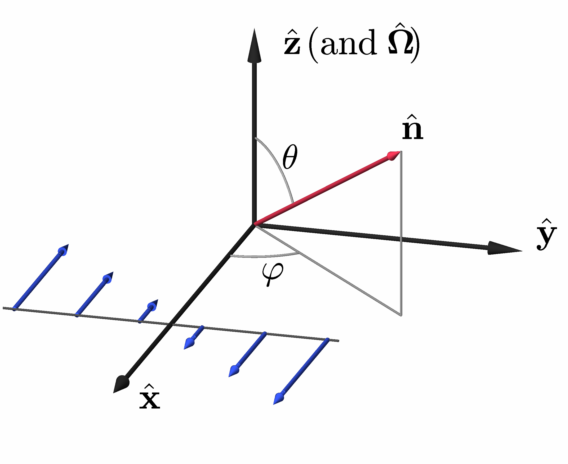
\includegraphics[width=7cm]{figs/fig_coordinates.png}}
\end{center}
\caption{\figlab{coordinates} }%
\end{figure}
\begin{figure}
\begin{center}
  \makebox[\textwidth]{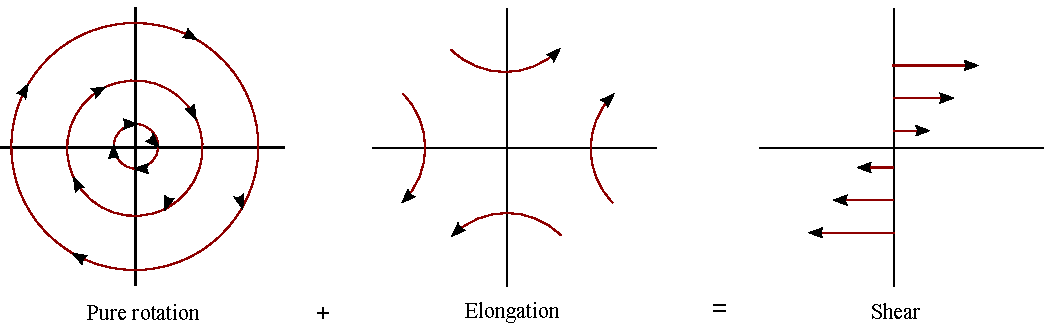
\includegraphics[width=1.2\textwidth]{figs/shear_decomposition}}
\end{center}
\caption{\label{fig:shear_decomposition} Decomposition of the simple shear flow.}%
\end{figure}


\section{The Jeffery equation and its solutions}\label{sec:jefferyequation}

In this section we consider axisymmetric particles: particles which are rotationally symmetric around an axis of symmetry. For such particles the orientational configuration may be represented by a unit vector $\ve n$, attached to the axis of symmetry. As alluded to in Sec.~\ref{sec:forces}, Jeffery presents two major results in his seminal paper from 1922 \cite{jeffery1922}. First, he calculates the hydrodynamic torque on a ellipsoid, not necessarily axisymmetric, in any linear flow. Second, he derives the equation of motion of an inertia-free, axisymmetric ellipsoid (a spheroid). This equation of motion is often referred to as the Jeffery equation. In our notation the Jeffery equation is
\begin{align}
	\dot{\ve n} &= \ma O \ve n + \Lambda \left(\ma S \ve n - \ve n \ve n \transpose \ma S \ve n\right).\eqnlab{jeffery}
\end{align}
Here $\ma O$ and $\ma S$ are the anti-symmetric and symmetric parts of the fluid gradient, as introduced in Sec.~\ref{sec:forces}. The parameter $\Lambda$ is a particle shape factor. For a spheroid of aspect ratio $\lambda$ the shape factor is
\begin{align*}
	\Lambda = \frac{\lambda^2-1}{\lambda^2+1}.
\end{align*}
For most conceivable particle shapes, $-1 < \Lambda < 1$. Negative $\Lambda$ correspond to flat, disk-shaped particles, while positive $\Lambda$ correspond to elongated, rod-like particles. It was shown by Bretherton \cite{bretherton1962} that, given the correct shape factor $\Lambda$, Jeffery's equation is valid not only for spheroids, but for any axisymmetric particle. He also showed that there are extreme cases where $|\Lambda|>1$. In this thesis we consider particles with $|\Lambda|<1$, like the spheroid.

 The equation of motion for an inertia-free particle is given by force and torque balance on the particle. Then the center-of-mass velocity equals the fluid velocity at the center-of-mass position, a condition called \emph{advection}. Jeffery's equation is the rotational analogue of center-of-mass advection. In Paper B, we demonstrate how to derive Jeffery's equation. We start from the hydrodynamic torque and Newton's equation of motion, and take the limit $\st\to 0$. In the following, we will instead consider the possible solutions of the Jeffery equation \eqnref{jeffery}.

Jeffery's equation is a non-linear vector equation, and as such it is seemingly hard to solve. However, the non-linearity is only apparent, it is due to the geometric constraint that $\ve n$ is a unit vector. The underlying dynamics is in fact linear. I will now explain two ways to understand this fact.

The vorticity $\ma O$ rotates $\ve n$, and the strain $\ma S$ aligns and stretches $\ve n$ towards its strongest eigendirection. The non-linear term $\ve n \ve n\transpose \ma S \ve n$ is simply the stretching component of the strain, which is subtracted in order to prevent elongation of $\ve n$. Bretherton (Sec.~6 in Ref.~\cite{bretherton1962}) realised that we may instead model the orientation of the particle with any vector $\ve q$ which obeys the same linear terms, but without compensating for any elongation:
\begin{align}
	\dot{\ve q} = \left(\ma O + \Lambda \ma S\right) \ve q.\eqnlab{jefferyq}
\end{align}
Owing to the common linear terms in \Eqnref{jeffery} and \Eqnref{jefferyq}, the vector $\ve q$ will have the same angular dynamics as $\ve n$. In addition, $\ve q$ may be stretched and compressed by the strain $\ma S$. But since we are only interested in the angular degrees of freedom, we can at any instant recover $\ve n$ by normalising $\ve q$ to unit length. Thus, the general solution of the Jeffery equation is given by solving \Eqnref{jefferyq} for $\ve q(t)$, then the solution to \Eqnref{jeffery} is given by normalising $\ve q(t)$ to unit length:
\begin{align}
	\ve n(t) &= \frac{\ve q(t)}{|\ve q(t)|}.\eqnlab{jefferysolution0}
\end{align}

Another, more mathematical, way of understanding how the linear companion equation \eqnref{jefferyq} arises is the following. Like above, we choose to represent the particle orientation by a vector $\ve q$ which is parallel to $\ve n$. Define $\ve q = \alpha(t)\ve n$, with $\alpha(t)$ an arbitrary function of time. We know from this definition that we may always recover $\ve n$ by normalising $\ve q$ to unit length. Now, we can calculate the equation of motion for $\ve q$:
\begin{align}
	\diff{\ve q}{t} &= \diff{}{t}\left(\alpha \ve n\right) \nn \\
	&= \dot \alpha \ve n + \alpha \dot{\ve n} \nn\\
	&= \dot \alpha \ve n + \alpha \left(\ma O \ve n + \Lambda \left(\ma S \ve n - \ve n \ve n \transpose \ma S \ve n\right)\right). \eqnlab{jefferyderivation1}
\end{align}
But $\alpha(t)$ is an arbitrary function which we may choose. In particular we can choose $\alpha(t)$ to be a function satisfying
\begin{align*}
	\dot \alpha &= \alpha \Lambda \ve n\transpose \ma S \ve n.
\end{align*}
By inserting this choice of $\alpha(t)$ into \Eqnref{jefferyderivation1}, we again arrive at \Eqnref{jefferyq}.

We will now consider the solutions of Jeffery's equation in time-independent flows. This case includes for example the simple shear flow, and indeed any linear flow. It is also a useful model when the flow changes only slowly in time, compared to the time it takes for the gradients to affect the particle orientation. First, I will describe the possible solutions of \Eqnref{Jeffery} in linear flows. This picture is vital in understanding our argument in Paper C (see also Sec.~\ref{sec:tumbling} in this thesis). Second, I will discuss the solutions of Jeffery's equation in a simple shear flow. The solutions are called the Jeffery orbits, and they play an important role in both Papers A and B.

When $\ma O$ and $\ma S$ are time-independent the linear companion equation \eqnref{jefferyq} is solved by the matrix exponential:
\begin{align*}
		\ve q(t) = e^{(\ma O + \Lambda \ma S)t}\ve q(0).
\end{align*}
This solution implies that the long-time dynamics of $\ve q$, and therefore $\ve n$, is determined by the eigenvalues and eigenvectors of the matrix $\ma B = \ma O + \Lambda\ma S$. For an incompressible flow $\tr\ma B=0$, because $\tr\ma A=0$. In other words, the three eigenvalues of $\ma B$ must sum to zero. Thus, there are three distinct possibilities for the eigensystem of $\ma B$:
\begin{enumerate}
	\item Three real eigenvalues, then
	\item[] $\ve q$ will align with the eigenvector corresponding to the largest eigenvalue.
	\item One real eigenvalue $a>0$, and a complex pair $-a/2 \pm i\omega$, then
	\item[] $\ve q$ will spiral into alignment with the eigenvector corresponding to the real eigenvalue.
	\item One real eigenvalue $a\leq0$, and a complex pair $-a/2 \pm i\omega$, then
	\item[] $\ve q$ will spiral out and rotate in the plane spanned by the real and imaginary parts of the complex eigenvector.
\end{enumerate}
\begin{figure}
\begin{center}
  \makebox[\textwidth]{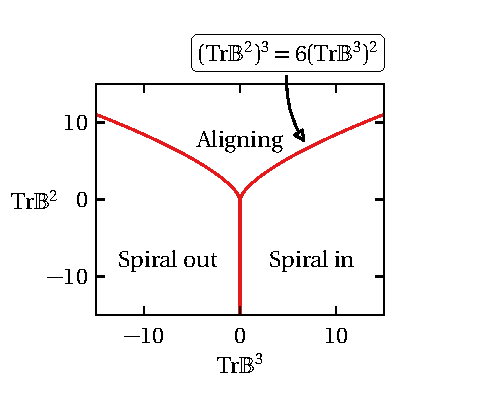
\includegraphics{figs/bmap}}
\end{center}
\caption{\label{fig:bmap} }%
\end{figure}
The characteristic equation for the eigenvalues $b$ of a $3\times3$-matrix $\ma B$ is
\begin{align*}
	-b^3 + \tr b^2\ma B  + \frac{b}{2}\left(\tr \ma B^2-(\tr \ma B)^2\right)+\det\ma B = 0.
\end{align*}
But for a traceless matrix $\tr \ma B=0$ and $\det \ma B = \tr\ma B^3/3$, thus
\begin{align}
	-b^3 + \frac{b}{2}\tr \ma B^2 +\frac{1}{3}\tr\ma B^3 = 0. \eqnlab{bcharacteristic}
\end{align}
It is possible to solve exactly for the eigenvalues, but the important observation is that they are determined by only two parameters: $\tr \ma B^2$ and $\tr\ma B^3$. In Fig.~\ref{fig:bmap} I illustrate how the three cases outlined above correspond to different values of $\tr \ma B^2$ and $\tr\ma B^3$. The boundary curve of the region of three real eigenvalues is given by the discriminant of the characteristic equation:
\begin{align*}
 	\Delta = \left(\tr \ma B^2\right)^3 - 6\left(\tr \ma B^3\right)^2 = 0.
 \end{align*} 
In the region where there is a pair of complex eigenvalues, the two cases of spiral in or out are separated by $\tr \ma B^3=0$. Now, what follows is one of the key observations in our argument in Paper C. For any given flow gradient, changing the particle from rod-like to disk-shaped (or vice versa) will transform $\tr \ma B^3\to-\tr\ma B^3$ and therefore change the qualitative dynamics from aligning to rotating (or vice versa). This transformation may be understood because
\begin{align*}
	\tr \ma B^3 = 3\Lambda \tr \ma O\ma O \ma S + \Lambda^3 \tr \ma S\ma S \ma S.
\end{align*}
The other combinations of $\ma S$ and $\ma O$ which could contribute, such as $\tr \ma O\ma O \ma O$, vanish identically because of symmetries of $\ma O$ and $\ma S$. As explained above, changing a particle from rod-like to disk-shaped implies a change of sign of the shape factor $\Lambda$. The implications of this observation for the tumbling of particles in turbulent and random flows are further discussed in Sec.~\ref{sec:tumbling} in Part~II, and in Paper C. 

The remainder of this section concerns the case of simple shear flow. This case is characterised by $\tr \ma B^3=0$ and $\tr \ma B^2<0$. The simple shear has a special position among flows, and we understand the significance of the condition $\tr\ma B^3=0$ from the above discussion. First, a change of particle shape does not change the qualitative dynamics. Both disk-shaped particles and rod-like particles rotate in a shear flow. Second, $\ma B$ has a zero eigenvalue, as seen from the characteristic equation \eqnref{bcharacteristic}. The zero eigenvalue is important, because it implies that the particle dynamics never forgets its initial condition. The eigenvector of the zero eigenvalue is the vorticity direction\footnote{See Fig.~\ref{fig:coordinates} and Sec.~\ref{sec:shearflow} for the definition of the coordinate system and the terminology of its directions in a simple shear flow.}, thus the component of $\ve q$ in the vorticity direction is constant in a shear flow. The other two eigenvalues are an imaginary pair, resulting in a periodic rotation of $\ve q$. In summary, the dynamics of $\ve q$ in a simple shear flow is a periodic rotation in a plane. The plane is normal to the vorticity direction, and determined by the initial condition of $\ve q$.

\begin{figure}
	\begin{center}
	  \makebox[\textwidth]{%
        \begin{subfigure}[b]{0.62\textwidth}
                \centering
                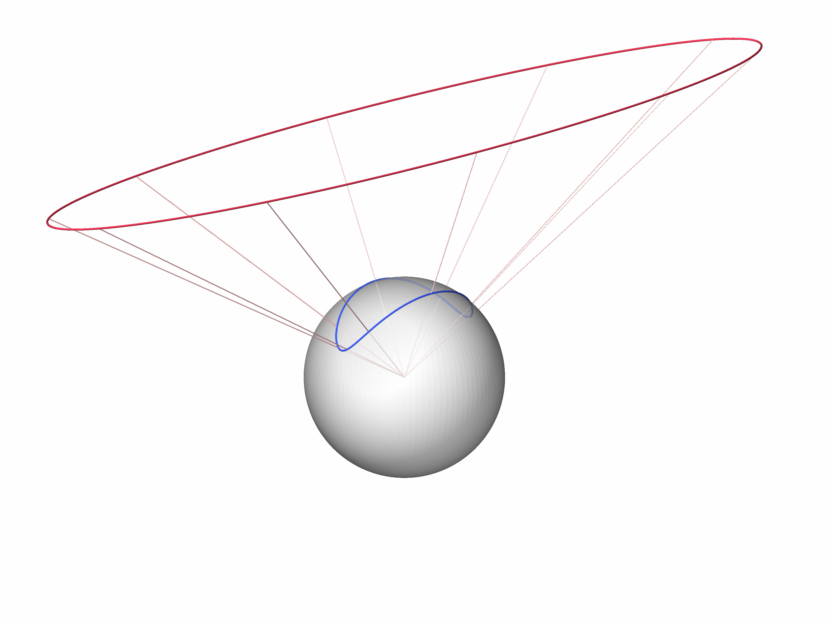
\includegraphics[width=\textwidth]{figs/projection_orbit1.png}
                \caption{}
                \label{fig:projection_orbit1}
        \end{subfigure}%
        \begin{subfigure}[b]{0.62\textwidth}
                \centering
                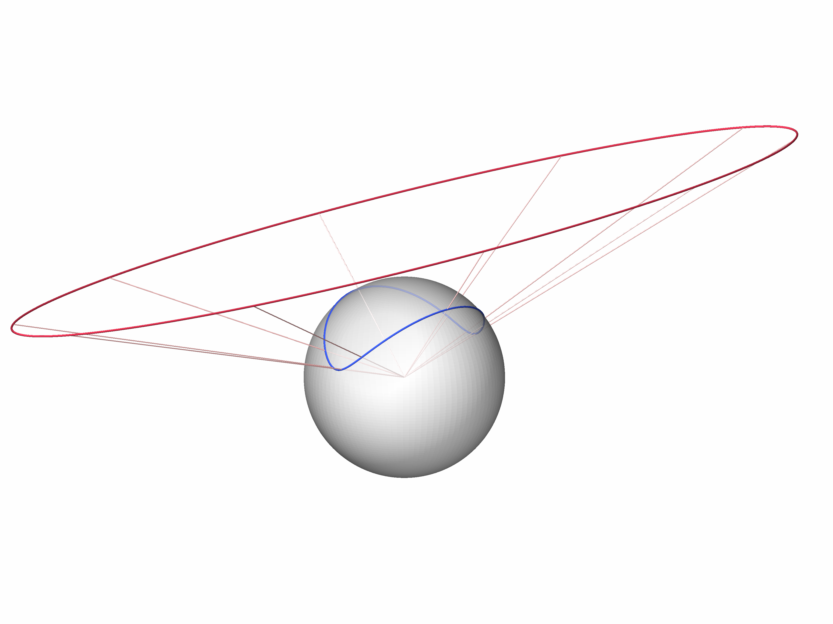
\includegraphics[width=\textwidth]{figs/projection_orbit2.png}
                \caption{}
                \label{fig:projection_orbit2}
        \end{subfigure}
        }
        \makebox[\textwidth]{%
        \begin{subfigure}[b]{0.62\textwidth}
                \centering
                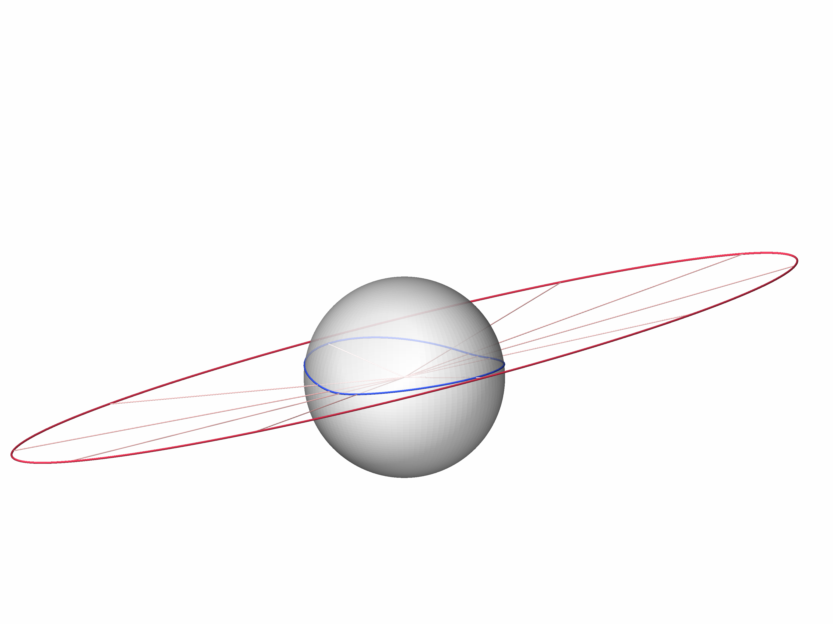
\includegraphics[width=\textwidth]{figs/projection_orbit3.png}
                \caption{}
                \label{fig:projection_orbit3}
        \end{subfigure}
        \begin{subfigure}[b]{0.62\textwidth}
                \centering
                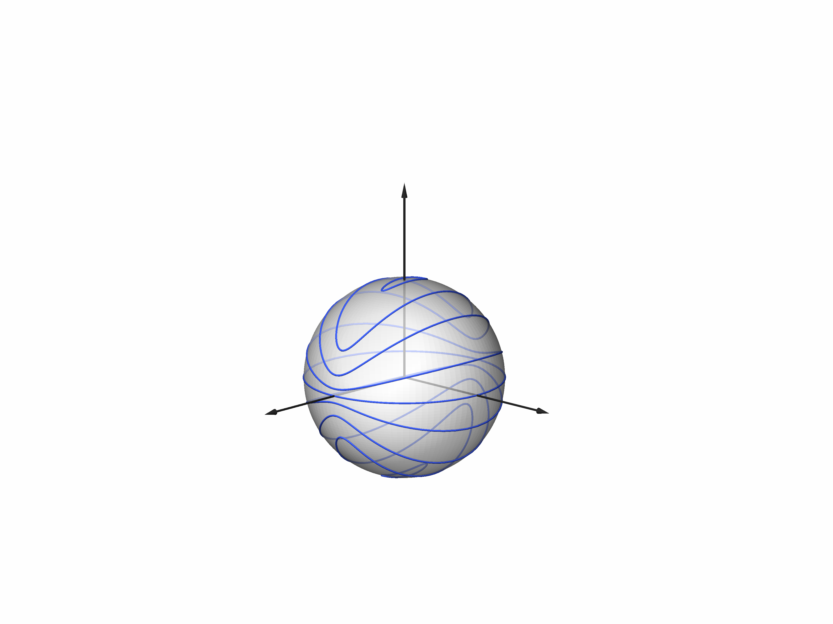
\includegraphics[width=\textwidth]{figs/projection_orbit4.png}
                \caption{}
                \label{fig:projection_orbit4}
        \end{subfigure}        
	  }%
	\end{center}
    \caption{\textbf{(a-c)} Illustrations of how the trajectories $\ve q(t)$ (red) produces the Jeffery orbits $\ve n(t)$ (blue) upon projection onto the unit sphere. \textbf{(d)} Sample of resulting Jeffery orbits with coordinate system. All trajectories correspond to a particle of aspect ratio $\lambda=5$ in a simple shear flow.}\label{fig:projection_orbits}
\end{figure}


The trajectories $\ve q(t)$ are projected onto the unit sphere, and the resulting $\ve n(t)$ are the Jeffery orbits. In Fig.~\ref{fig:projection_orbits} the trajectories $\ve q(t)$ and $\ve n(t)$ are illustrated for particle aspect ratio $\lambda=5$, and three different initial conditions.

The solutions to Jeffery's equation in a simple shear flow are degenerate: the orientational trajectory depends on the initial condition for all time. In many realistic situations this long-time memory hardly seems plausible. The assumptions leading up to Jeffery's equation and its periodic solution each correspond to a physical mechanism that may or may not break the degeneracy. The three assumptions we believe most important to investigate are the following.

First, the particle may not be axisymmetric. In this case the dynamics is more complicated, but still depends on initial condition. Tri-axial particles are discussed further in relation to Paper A in Sec.~\ref{sec:experiment}.

Second, there may be inertial effects. Fluid inertia was neglected when we used the resistance tensor formulation \eqnref{resistanceformulation} for the torque on a particle. Particle inertia was neglected when Newton's equation reduced to Jeffery's equation in the advective limit $\st \to 0$. In Paper B we describe how the effects of a small amount of particle inertia break the degeneracy of the solutions $\ve n(t)$. See the discussion in \ref{sec:inertia} for an outlook on the case of fluid inertia.

Finally, the third mechanism is Brownian noise. The idea is that thermal fluctuations kicks the particle out of one Jeffery orbit and into another. After some time, the initial condition is forgotten and the state of the particle is described by an orientational probability distribution. The problem of computing the orientational distribution has a long history, and in the next Section I briefly review some of the methods and results.

\section{Orientational distributions}\seclab{orientationaldistributions}

In this Section we consider the orientational dynamics of an axisymmetric particle, represented by the vector $\ve n$. In this case the orientational distribution is a function $P(\ve n, t)$ which describes the probability of observing the particle with orientation\footnote{Strictly, $P(\ve n, t)\rd S$ is the probability to find $\ve n$ on the surface element $\rd S$ at time $t$.} $\ve n$ at time $t$. Instead of asking for the orientational trajectory $\ve n(t)$ of a particle given the initial condition $\ve n(0)$, we now ask what the orientational distribution $P(\ve n, t)$ is, given the initial condition $P(\ve n, 0)$.

By far the most common approach is to consider a diffusion equation for the unit vector $\ve n$. My simplistic view of the diffusion approximation is the following. The orientation of the particle is driven by very many, very small and very fast kicks. In the case of particles in fluids, the small kicks originate in the bombardment of fluid molecules onto the particle surface. These \emph{microscopic} kicks are so small and fast that we never see them directly. But after a short time, enough kicks have accumulated into an observable change. If we reset the particle orientation and start over, the microscopic kicks will again accumulate into an observable change. But because the molecular bombardment is not exactly the same every time, the accumulated change is different every time. The diffusion approximation is to not consider all the details of the random kicks, but to only consider the \emph{mean value} and \emph{variance} of the accumulated changes. The idea is to replace the complicated accumulation of microscopic kicks with randomly chosen changes. The randomly chosen steps will have the correct mean value and variance, but all other details are neglected. The idea is based mathematically in the Central Limit Theorem of statistics, stating that if you add many random numbers the sum will converge to be normally distributed (under certain conditions). For a complete and very readable account of the method I point to the book \emph{Stochastic Processes in Physics and Chemistry}, by van Kampen \cite{kampen2007}.

The governing equation for the orientational distribution of an axisymmetric particle in the diffusion approximation is the Fokker-Planck equation
\begin{align}
	\frac{\partial}{\partial t}P(\ve n, t) &= \frac{\partial}{\partial \ve n}\left[\ve J (\ve n, t)P(\ve n, t)\right] + \mathcal D \frac{\partial^2}{\partial \ve n^2}P(\ve n, t).\eqnlab{fpejeff}
\end{align}
The first term on the right hand side is referred to as the drift, and the second as the diffusion. The drift is due to the deterministic fluid flow, and $\ve J(\ve n, t)$ represents the right hand side of the Jeffery equation \eqnref{jeffery}. The diffusion term is due to the random kicks, and $\mathcal D$ is the rotational diffusion constant. Since $\ve n$ is a unit vector, the Fokker-Planck equation is defined on the unit sphere. Therefore the derivative with respect to $\ve n$ is defined as $\partial/\partial_{\ve n} = (\ma I-\ve n\ve n\transpose)\nabla$, with $\nabla$ the usual gradient in $\mathbb R^3$. In Appendix~\secref{fpesphere} I explain this in more detail, and present a full derivation of \Eqnref{fpejeff}. 

For the purposes of this thesis, and more specifically in understanding Paper B, we consider the case when a particle is suspended in a simple shear flow, and at the same time subject to Brownian noise. As mentioned in the previous Section, the solutions to Jeffery's equation in a simple shear flow are degenerate. The orientational distribution of $\ve n$ under the influence of, for example, thermal noise has been extensively studied, as a means of explaining how particles in shear ``forget'' their initial conditions. A thorough review is given in \cite{brenner1974}, and what follows is a brief summary.

The dynamics is governed by a single dimensionless parameter, the P\'eclet number $\pe = s/\mathcal D$. Here $\mathcal D$ is the diffusion constant in \Eqnref{fpejeff}, and $s$ is the shear strength, or the strength of the drift term in \Eqnref{fpejeff}. A small value of $\pe$ means that the noise is strong, and vice versa. 

\begin{figure}
\begin{center}
  \makebox[\textwidth]{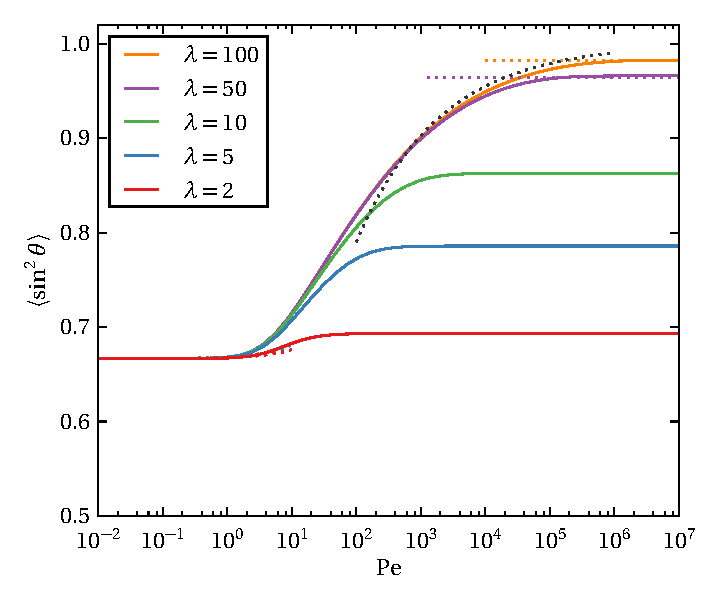
\includegraphics{figs/sintheta1.pdf}}
\end{center}
\caption{\figlab{sintheta1} Stationary average $\langle \sin ^2\theta \rangle$ for an axisymmetric particle in a shear flow subject to random noise, shown as function of the P\'eclet number $\pe = s/\mathcal D$ for different values of the particle aspect ratio $\lambda$. Larger $\pe$ corresponds to less noise. Solid lines are numerical solutions. Dotted lines show asymptotes in regimes of weak, intermediate and strong noise, compiled in \cite{brenner1974}.}%
\end{figure}

For small $\pe$, when the noise dominates, the orientational distribution is uniform - all orientations are equally likely. When the noise is decreased, the orientational distribution begins to reflect the Jeffery orbits. As $\pe$ becomes larger and the shear grows increasingly important, the probability of seeing a particle aligned with the flow direction increases. 
But surprisingly, when $\pe$ becomes large enough, the stationary orientational distribution converges and becomes \emph{independent of} $\pe$. In other words, when the noise is small enough, the particles follow the Jeffery orbits, but every now and then jump to a different orbit.

The stationary orientational distribution depends on the value of $\pe$ and the particle aspect ratio $\lambda$. In order to quantify the above discussion, I show numerical solutions\footnote{The details of how I solve \Eqnref{fpejeff} numerically can be found in Appendix~\ref{app:fpe_sphere}.} for the stationary average $\langle \sin^2\theta \rangle$ in \Figref{sintheta1}. The angle $\theta$ is the polar angle of $\ve n$, such that $n_z = \cos\theta$. It is also the angle to the vorticity direction, see \Figref{coordinates}. 

For small $\pe$ we see that $\langle \sin^2\theta \rangle = 1/3$. But for large $\pe$, the average reaches a plateau, depending on particle aspect ratio $\lambda$. The asymptotic solutions of \Eqnref{fpejeff} described in \cite{brenner1974} are shown as dotted lines. In particular, Hinch \& Leal \cite{hinch1972} solved the mathematically involved problem of weak noise. They obtained an expression for the height of the plateau valid for thin particles, $\lambda\gg1$. The numerical solution confirms their prediction.

In Paper B we compute the same orientational average, $\langle \sin^2\theta \rangle$, when the particle has a small but finite mass, as characterised by the Stokes number.



\end{document}
